\documentclass[../distribution_theory_notes.tex]{subfiles}
\begin{document}
\section{Aula 04 - 26 de Agosto, 2025}
\subsection{Motivações}
\begin{itemize}
	\item Mais Exemplos;
	\item Notação Multi Índices;
	\item Convergência em Compactos;
	\item Suporte de Funções Contínuas.
\end{itemize}
\subsection{Convergência em Compactos e Suporte de Funções Contínuas}
Com as ferramentas desenvolvidas ao longo da última aula, seremos capazes de descrever todos os espaços das funções usadas na Teoria das Distribuições, as chamadas \textit{funções testes}. Começaremos isto nessa aula, utilizando exemplos para adicionar conceitos que serão utilizados ao longo do processo.
\begin{example}[Espaço \(\mathcal{C}(\Omega )\)]
	Seja \(\Omega \) um aberto qualquer de \(\mathbb{R}^{N}\) e consideremos o conjunto
	\[
		\mathcal{C}(\Omega )=\mathcal{C}(\Omega ; \mathbb{C})\coloneqq \{f:\Omega \rightarrow \mathbb{C}:\; f\text{ é contínua.}\}
	\]
	Fixada uma exaustão qualquer de \(\Omega \), digamos \((K_{j})_{j\in \mathbb{N}},\) definimos para cada j natural
	\begin{align*}
		p_{j}: & \mathcal{C}(\Omega )\rightarrow \mathbb{R}          \\
		       & f\mapsto p_{j}(f)\coloneqq \sup_{x\in K_{j}}|f(x)|.
	\end{align*}
	\begin{figure}[H]
		\begin{center}
			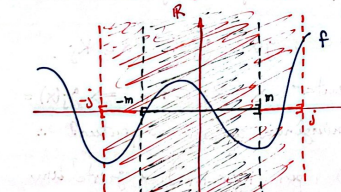
\includegraphics[height=0.5\textheight, width=0.5\textwidth, keepaspectratio]{./Images/continuous_space_seminorm_04.png}
		\end{center}
		\caption{a seminorma \(p_{j}\) só vê o comportamento de f sobre \(K_{j}\); além disso, \(p_1(f)\leq p_2(f)\leq \dotsc \leq p_{j}(f)\leq \dotsc \)}
	\end{figure}

	Para todo f em \(\mathcal{C}(\Omega )\) e j natural, \(p_{j}(f) < \infty\), indicando que \(p_{j}\) está bem definido. Além disso, a família \(\{p_{j}\}_{j\in \mathbb{N}}\) é separante, pois, se f for não nula, então existe um ponto \(x_{0}\) de \(\Omega \) com \(f(x_{0})\) também não nula. Logo, existe \(j_{0}\) natural tal que
	\[
		x_{0}\in K_{j_{0}} \Rightarrow p_{j}(f)\geq |f(x_{0})|>0
	\]
	e, por ser enumerável, \(\mathcal{C}(\Omega )\) é um TVS localmente convexo e metrizável quando munido da topologia gerada por \(\{p_{j}\}_{j\in \mathbb{N}}\). \textbf{Sempre que nos referirmos a \(\mathcal{C}(\Omega )\) como um TVS, estaremos admitindo que ele está munido desta topologia.}

	Vejamos o tipo de convergência é descrita por esta topologia! Considere \(\{f_{n}\}_{n\in \mathbb{N}}\) e f uma função em \(\mathcal{C}(\Omega )\) com \(f_{n}\substack{\mathcal{C}(\Omega ) \\ \rightarrow \\ }f\). Do lema da aula passada, isto significa que, para todo j natural,
	\[
		p_{j}(f_{n}-f)\substack{ \\ \rightarrow \\ n\to \infty}0 \Leftrightarrow \sup_{x\in K_{j}}|f_{n}(x)-f(x)|\substack{ \\ \rightarrow \\ n\to \infty}0.
	\]
	Assim, a convergência de \(\{f_{n}\}_{n}\) até f é uniforme em cada \(A_{j}\) da exaustão, mas isto basta para a \textit{convergência uniforme em cada compacto} K contido em \(\Omega \), pois
	\[
		K\subseteq \bigcup_{j=1}^{\infty}\mathrm{int}(K_{j})\Rightarrow K\subseteq \mathrm{int}(K_{j_1})\cup \dotsc \cup \mathrm{int}(K_{j_p})\Rightarrow K\subseteq K_{j_{0}}
	\]
	Se \(j_{0}\) for o máximo dos valores de \(j_1,\dotsc \Psi _{p}\), então
	\[
		\sup_{K}|f_{n}(x)-f(x)|\leq \sup_{K_{j_{0}}}|f_{n}(x)-f(x)|\substack{ \\ \rightarrow \\ n\to \infty}0.
	\]
	Além disso, toda sequência de Cauchy em \(\mathcal{C}(\Omega )\) converge, tendo em vista que uma sequência de funções \(\{f_{n}\}_{n}\) ser de Cauchy em \(\mathcal{C}(\Omega )\) equivale a dizer que a sequência de suas restrições \(\{f_{n}|_{K_{j}}\}_{n}\) é de Cauchy para cada j. Como \(\mathcal{C}(K_{j})\) é completo com a \textit{norma do supremo}, ou seja,
	\[
		\Vert g \Vert_{(u, j)}=\sup_{K_{j}}|g(x)|
	\]
	para cada j natural, existe um \(g_{j}\) em \(\mathcal{C}(K_{j})\) tal que
	\[
		f_{n}|_{K_{j}}\substack{\Vert \cdot  \Vert_{(u, j)} \\ \rightarrow \\ }g_{j}
	\]
	Nestas condições, definimos a função \(g:\Omega \rightarrow \mathbb{C}\) pondo, para cada x em \(K_{j}\), \(g(x)\coloneqq g_{j}(x);\) desta forma, note que, se x é um ponto em \(K_{j}\cap K_{r}\), onde r é maior que j, então
	\[
		x\in K_{j}\subseteq K_{r}\Rightarrow g_{j}(x)=g_{r}(x)
	\]
	pela unicidade do limite, tornando g bem definida. Para finalizar, como \(g|_{\mathrm{int}(K_{j})}\) é contínua para todo j natural, concluímos que \(g\in \mathcal{C}(\Omega )\) e, para j natural,
	\[
		p_{j}(f_{n}-g)=\sup_{K_{j}}|f_{n}(x)-g(x)|=\sup_{K_{j}}|f_{n}(x)-g_{j}(x)|\substack{ \\ \rightarrow \\ n\to \infty}0.
	\]
	Portanto, \(f_{n}\substack{\mathcal{C}(\Omega ) \\ \rightarrow \\ }f\) e \(\mathcal{C}(\Omega )\) é \textit{sequencialmente completo}.
\end{example}
\begin{example}[Espaço \(\mathcal{H}(\Omega )\)]
	Neste caso, se \(\Omega \) é visto como um subconjunto de \(\mathbb{C}\) identificado com \(\mathbb{R}^{2}\), seja
	\[
		\mathcal{H}(\Omega )\coloneqq \{f:\Omega \rightarrow \mathbb{C}:\; f \text{ é holomorfa em }\Omega \}.
	\]
	Como \(\mathcal{H}(\Omega )\) é um subconjunto de \(\mathcal{C}(\Omega )\), podemos considerá-lo como um espaço munido da topologia da convergência uniforme em compactos induzida por \(\mathcal{C}(\Omega )\). Além disso, um resultado conhecido é que o limite uniforme em compactos de uma sequência de funções holomorfas é em si uma função holomorfa. Portanto, \(\mathcal{H}(\Omega )\) é um subespaço fechado de \(\mathcal{C}(\Omega )\), consequentemente tornando-o sequencialmente completo. Daqui adiante, sempre será admitido que \(\mathcal{H}(\Omega )\) está munido desta topologia.
\end{example}
\begin{example}[Espaço \(L_{\mathrm{loc}}^{p}(\Omega )\)]
	Fixados \(\Omega \) um aberto qualquer de \(\mathbb{R}^{N}\) munido da \(\sigma\)-álgebra de Borel ou Lebesgue e da medida de Lebesgue, p um valor do tipo \(1\leq p\leq \infty\), e \(\{K_{j}\}_{j}\) uma exaustão de \(\Omega \), definimos
	\[
		L_{\mathrm{loc}}^{p}(\Omega )\coloneqq \{f:\Omega \rightarrow \mathbb{C}:\; f \cdot \chi_{K}\in L^{p}(K) \;\forall\; K\subseteq \Omega \text{ compacto e }f\text{ é mensurável}\},
	\]
	além da família de seminormas determinadas pela regra
	\[
		p_{j}(f)\coloneqq \Vert f \cdot \chi_{K_{j}} \Vert_{p} = \left\{\begin{array}{ll}
			\biggl(\int_{K_{j}}^{}|f(x)|^{p} \mathrm{dx}\biggr)^{\frac{1}{p}}, & \quad 1\leq p< \infty \\
			\mathrm{sup\;ess}_{x\in K_{j}}|f(x)|,                              & \quad p=\infty
		\end{array}\right.,
	\]
	onde \(\chi_{B}:\mathbb{R}^{N}\rightarrow \mathbb{R}\) é a função característica de B, isto é,
	\[
		\chi_{B} = \left\{\begin{array}{ll}
			1, & \quad x\in B     \\
			0, & \quad x\not\in B \\
		\end{array}\right.
	\]
	e ``sup ess'' é o \textit{supremo essencial}, dado por
	\[
		\mathrm{sup\; ess}_{x\in B}|g(x)| \coloneqq \inf_{}\{\alpha >0:\; m(\{x\in B:\; |f(x)|>\alpha \})=0\}.
	\]
	\begin{figure}[H]
		\begin{center}
			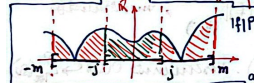
\includegraphics[height=0.5\textheight, width=0.5\textwidth, keepaspectratio]{./Images/locp_seminorms_04.png}
		\end{center}
		\caption{aumentando o j, capturamos mais massa: \(p_{j}(f)\leq p_{j+1}(f)\).}
	\end{figure}

	Dito isso, vamos estudar a noção de convergência neste espaço para os casos onde p é um valor finito, deixando o restante como exercício para o leitor. Segue da desigualdade de Minkowski que cada \(p_{j}\) é uma seminorma em \(L_{\mathrm{loc}}^{p}(\Omega )\) e, além do mais, a sequência formada por elas é saparante, tendo em vista que se f não é identicamente nula em \(L_{\mathrm{loc}}^{p}(\Omega )\), existirá um subconjunto E de \(\Omega \) que é limitado, \(f\) é não nula em E, e \(m(E)>0\); sendo m ``regular por dentro'', existe um compacto \(K\subseteq E\) com \(m(K)>0\), tal que, tomando \(K_{j}\supseteq K\), quando p for finito,
	\[
		\int_{K_{j}}^{}|f(x)|^{p} \mathrm{dx}\geq \int_{K}^{}|f(x)|^{p} \mathrm{dx}>0 \text{(Verifique!\footnote{Dica: podemos escolher E tal que \(|f|\geq 1/m>0\) em E, pois m é \(\sigma \)-finita.}}
	\]
	Desta forma, \(L_{\mathrm{loc}}^{p}(\Omega )\) é um TVS localmente convexo e metrizável quando munido da topologia gerada pela sequência de seminormas \(\{p_{j}\}_{j\in \mathbb{N}}.\)

	Quanto à convergência (tendo em vista que vale uma versão de convergência dominada no espaço em que estamos), se \(f_{n}\substack{L_{\mathrm{loc}}^{p} \\ \rightarrow \\ }f\), então para todo j,
	\[
		p_{j}(f_{n}-f)\substack{n\to \infty \\ \rightarrow \\ }0,
	\]
	ou seja, para todo j natural,
	\[
		\int_{K_{j}}^{}|f_{n}(x)-f(x)|^{p} \mathrm{dx}\substack{n\to \infty \\ \rightarrow \\ }0.
	\]
	Assim como no exemplo anterior, isto é suficiente para garantir que a convergência de \(L_{\mathrm{loc}}^{p}\) é a convergência em \(L^{p}\) para cada compacto de \(\Omega \). Finalmente, sendo cada \(L_{\mathrm{loc}}^{p}(K_{j})\) um espaço de Banach, é possível provar que \(L_{\mathrm{loc}}^{p}\) é também sequencialmente completo, também deixado como exercício.
\end{example}
\begin{tcolorbox}[
		skin=enhanced,
		title=Observação,
		fonttitle=\bfseries,
		colframe=black,
		colbacktitle=cyan!75!white,
		colback=cyan!15,
		colbacklower=black,
		coltitle=black,
		drop fuzzy shadow,
		%drop large lifted shadow
	]
	Ao considerarmos o espaço \(L_{\mathrm{loc}}^{p}(\Omega )\) como TVS, admitiremos que a topologia é a dada acima, a qual independe da exaustão escolhida. Ademais, quando \(p=1\), dizemos que \(L_{\mathrm{loc}}^{1}(\Omega )\) é o \textbf{\textit{espaço das funções localmente integráveis}} e, no caso geral, é o espaço das funções \textbf{\textit{localmente \(L^{p}\)}}.
\end{tcolorbox}
\begin{tcolorbox}[
		skin=enhanced,
		title=Observação,
		fonttitle=\bfseries,
		colframe=black,
		colbacktitle=cyan!75!white,
		colback=cyan!15,
		colbacklower=black,
		coltitle=black,
		drop fuzzy shadow,
		%drop large lifted shadow
	]
	Para todo \(1\leq p\leq \infty\), vale \(\mathcal{C}(\Omega )\subseteq L_{\mathrm{loc}}^{p}(\Omega )\); além do que, para todo j e \(1\leq p\leq \infty\),
	\[
		\biggl(\int_{K_{j}}^{}|f(x)|^{p} \mathrm{dx}\biggr)^{\frac{1}{p}}\leq m(K_{j})^{\frac{1}{p}}\Vert f \Vert_{(u, j)},
	\]
	mostrando que a inclusão é contínua. Escrevemos, assim,
	\[
		\mathcal{C}(\Omega )\hookrightarrow L_{\mathrm{loc}}^{p}(\Omega ).
	\]

	Com essa notação, no caso em que \(1\leq p\leq q\leq \infty\), vale a relação \(L_{\mathrm{loc}}^{q}(\Omega )\hookrightarrow L_{\mathrm{loc}}^{p}(\Omega )\) em virtude da Desigualdade de Hölder.
\end{tcolorbox}

\begin{def*}
	Dado m natural, considere o conjunto
	\[
		\mathbb{Z}_{+}^{n}=\{\alpha = (\alpha_1, \alpha_2, \dotsc , \alpha_{n}):\; \alpha_{j}\in \mathbb{N}\;\&\; \alpha_{j}\geq 0,\; j=1,2,\dotsc ,n\}.
	\]
	Os elementos de \(\mathbb{Z}_{+}^{n}\) serão chamados \textbf{multi-índices.} Escreveremos:
	\begin{itemize}
		\item \(|\alpha |=\alpha_1+\alpha_2+\dotsc +\alpha_{n}\) e chamaremos \textbf{ordem}, ou \textbf{tamanho}, ou ainda \textbf{comprimento} de \(\alpha\);
		\item \(\alpha! = \alpha_1!\alpha_2!\dotsc \alpha_{n}!\) é o \textbf{fatorial de} \(\alpha \);
		\item Se \(x=(x_1,\dotsc ,x_{n})\in \mathbb{R}^{n}\) e \(\alpha\in \mathbb{Z}_{+}^{n},\) então \(x^{\alpha }=x_{1}^{\alpha_1}\dotsc x_{n}^{\alpha_{n}}\);
		\item Escrevendo \(\partial_{j}=\frac{\partial^{}}{\partial x_{j}^{}}\) para a derivada parcial com relação à variável \(x_{j}\). Poremos, também,
		      \[
			      \partial_{j}^{\alpha_{j}}=\frac{\partial^{\alpha_{j}}}{\partial x_{j}^{\alpha_{j}}}
		      \]
		      para simbolizar que derivamos \(\alpha_{j}\) vezes a variável \(x_{j}\), onde \(\alpha_{j}\geq 0\) é inteiro, e então, para \(\alpha \in \mathbb{Z}_{+}^{n},\)
		      \[
			      \partial^{\alpha } = \frac{\partial^{\alpha_1}}{\partial x_1^{\alpha_1}}\circ \frac{\partial^{\alpha_2}}{\partial x_2^{\alpha_2}}\circ\cdots\circ \frac{\partial^{\alpha_n}}{\partial x_n^{\alpha_n}}
		      \]
		      como composição de aplicações lineares; note que \(\partial^{\alpha }\) é uma \textbf{derivada parcial de ordem \(|\alpha |\)};
		\item Finalmente, poremos
		      \[
			      D^{\alpha }\coloneqq \frac{1}{(2\pi i)^{|\alpha |}}\partial^{\alpha }.\;\square
		      \]
	\end{itemize}
\end{def*}

\begin{example}[Espaço \(\mathcal{C}^{\infty}(\Omega )\)]
	Como antes, fixaremos um aberto \(\Omega \) de \(\mathbb{R}^{N}\). Com isso, seja
	\[
		\mathcal{C}^{\infty}(\Omega )=\mathcal{C}^{\infty}(\Omega ; \mathbb{C})\coloneqq \{f:\Omega \rightarrow \mathbb{C}:\; f \text{ é infinitamente diferenciável em }\Omega \},
	\]
	que pode ser reescrito como
	\[
		\mathcal{C}^{\infty}(\Omega )=\bigcap_{m=0}^{\infty}\mathcal{C}^{m}(\Omega ),
	\]
	onde, para cada \(m\in \mathbb{Z}_{+}\),
	\[
		\mathcal{C}^{m}(\Omega )=\{f:\Omega \rightarrow \mathbb{C}:\; \partial^{\alpha }f \text{ existe e é contínua em }\Omega,\; |\alpha |\leq m,\; \alpha \in \mathbb{Z}_{+}^{n}\}
	\]
	é o espaço das funções complexas definidas em \(\Omega \) e de classe \(\mathcal{C}^{m}\), ou seja, que são m-vezes continuamente diferenciáveis.

	A partir disso, se \(\{K_{j}\}_{j}\) é um esgotamento qualquer de \(\Omega \), definimos, para cada j e m, os seguintes membros da família de seminormas:
	\begin{align*}
		p_{(m, j)}: & \mathcal{C}^{\infty}(\Omega )\rightarrow \mathbb{R}                                                                \\
		            & f \mapsto p_{(m, j)}(\varphi )\coloneqq \sum\limits_{|\alpha |\leq m}^{}\sup_{x\in K_{j}}|\partial^{\alpha }f(x)|,
	\end{align*}
	que, em particular, gera a mesma seminorma do exemplo 2 quando m vale 0, ou seja, \(p_{(0, j)}=p_{j}\) do exemplo 2. Isso facilita ver que \(\mathcal{C}^{\infty}(\Omega )\) é um TVS localmente convexo e metrizável quando munido da topologia gerada por esta família, já que ganhamos a enumeração e a propriedade separante. Como de costume, estaremos supondo que \(\mathcal{C}^{\infty}(\Omega )\) possui essa topologia quando aparecer.

	Com relação à sua convergência, observe que, se
	\[
		f_{n}\substack{\mathcal{C}^{\infty} \\ \rightarrow \\ }f,
	\]
	então
	\[
		p_{(m, j)}(f_{n}-f)\substack{ \\ \rightarrow \\ n\to \infty}0,\; \forall m,\; j,
	\]
	ou seja,
	\[
		\sum\limits_{|\alpha |\leq m}^{}\sup_{x\in K_{j}}|\partial^{\alpha }f_{n}(x)-\partial^{\alpha }f|\substack{ \\ \rightarrow \\ n\to \infty}0,
	\]
	o que quer dizer exatamente que, para todo \(|\alpha |\leq n\), vale
	\[
		\partial^{\alpha }f_{n}\substack{ \\ \rightarrow \\ }\partial^{\alpha }f
	\]
	em \(\mathcal{C}(\Omega )\), o que significa que todas as derivadas parciais de \(f_{n}\) convergem uniformemente para as derivadas correspondentes de f em compactos de \(\Omega \) quando n tende a infinito.

	Para ver que \(\mathcal{C}^{\infty}(\Omega )\) é sequencialmente compacto, considere uma sequência de Cauchy \(\{f_{n}\}_{n}\). Logo, para todo \(\alpha \), a sequência \(\{\partial^{\alpha }f_{n}\}_{n}\) é Cauchy em \(\mathcal{C}(\Omega )\), o qual já sabemos ser completo. Consequentemente, para cada \(\alpha \) em  \(\mathbb{Z}_{+}^{n},\) existe uma função \(g_{\alpha }\in \mathcal{C}(\Omega )\) com
	\[
		\partial^{\alpha }f_{n}\substack{\mathcal{C}(\Omega ) \\ \rightarrow \\ n\to \infty}g_{\alpha }.
	\]
	Nessas condições, seja \(f:\Omega \rightarrow \mathbb{C}\) dada por \(f\coloneqq g_{(0,0,\dotsc ,0)},\) a qual é contínua.

	\textbf{\underline{Afirmação}:} \(f\in \mathcal{C}^{\infty}(\Omega )\) para todo \(\alpha \in \mathbb{Z}_{+}^{n}\) e \(\partial^{\alpha }f = g_{\alpha }\).

	Para provarmos esta afirmação, podemos fazer uso do princípio da indução: com efeito, se \(|\alpha |=1,\) então
	\[
		\alpha  = e_{k}=(0,0,\dotsc ,0,\underbrace{1}_{\mathclap{\text{k-ésima posição}}},0,\dotsc ,0).
	\]
	Fixemos x em \(\Omega \) e j natural com \(x\in \mathrm{int}(K_{j})\). Pelo Teorema Fundamental do Cálculo, podemos escrever, para \(t\neq 0\) pequeno e n natural qualquer,
	\[
		f_{n}(x+te_{k})-f_{n}(x)=\int_{0}^{t}\frac{\partial^{}f_{n}}{\partial x_{k}^{}}(x+se_{k}) \mathrm{ds}\substack{n\to \infty \\ \rightarrow \\ }f(x+te_{k})-f(x)=\int_{0}^{t}g_{e_{k}}(x+se_{k}) \mathrm{ds},
	\]
	pois, no compacto \([x-\delta e_{k}, x+\delta e_{k}]\subseteq \mathrm{int}(K_{j})\), temos
	\[
		\frac{\partial^{}f_{n}}{\partial x_{k}^{}}\substack{n\to \infty \\ \rightarrow \\ \alpha =e_{k} }g_{e_{k}},
	\]
	mostrando que podemos trocar o limite com a integral. Assim, usando mais uma vez o TFC,
	\[
		\lim_{t\to 0} \frac{f(x+te_{k})-f(x)}{t} = \lim_{t\to 0}\frac{1}{t}\int_{0}^{t}g_{e_{k}}(x+se_{k}) \mathrm{ds} = g_{e_{k}}(x),
	\]
	isto é,
	\[
		\frac{\partial^{}f}{\partial x_{k}^{}} = g_{e_{k}}.
	\]
	Aplicando indutivamente este argumento no \(|\alpha |\), segue a prova da afirmação. \(\blacktriangle \)

\end{example}
\begin{tcolorbox}[
		skin=enhanced,
		title=Observação,
		fonttitle=\bfseries,
		colframe=black,
		colbacktitle=cyan!75!white,
		colback=cyan!15,
		colbacklower=black,
		coltitle=black,
		drop fuzzy shadow,
		%drop large lifted shadow
	]
	Dado \(\alpha \) em \(\mathbb{Z}_{+}^{n}\) e supondo que, para todo \(|\alpha |\leq m\), temos \(\partial^{\alpha }f = g_{\alpha }\), então seja \(\alpha \) com \(|\alpha |=m+1\), tal que \(\alpha = \beta +e_{k}\) para algum \(|\beta |=m\) e \(k = 1,2,\dotsc ,n.\) Assim, escrevendo
	\[
		\partial^{\beta }f_{n}(x+te_{k})-\partial^{\beta }f_{n}(x)=\int_{0}^{t}\frac{\partial^{}}{\partial x_{k}^{}}(\partial^{\beta }f_{n})(x+se_{k}) \mathrm{ds}
	\]
	e repetindo o argumento, obtemos
	\[
		\partial^{\beta }f(x+te_{k})-\partial^{\beta }f(x)=\int_{0}^{t}g_{\beta +e_{k}}(x+se_{k}) \mathrm{ds},
	\]
	que nos dá
	\[
		\frac{\partial^{}}{\partial x_{k}^{}}(\partial^{\beta }f)(x)=g_{\beta+e_{k}},
	\]
	ou seja,
	\[
		\partial^{\alpha }f = g_{\alpha },\quad |\alpha |=m+1.
	\]

	Em particular, como \(p_{(m, j)}(f)\leq p_{j}(f)\) para todos m e j, temos a relação \(\mathcal{C}^{\infty}(\Omega )\hookrightarrow \mathcal{C}(\Omega )\).
\end{tcolorbox}
\begin{example}[O Espaço de Schwartz \(\mathcal{S}=\mathcal{S}(\mathbb{R}^{n})\)]
	Para cada N natural e \(\alpha \) em \(\mathbb{Z}_{+}^{n},\) seja, para f em \(\mathcal{C}^{\infty}=\mathcal{C}^{\infty}(\mathbb{R})\), a quantidade
	\[
		\Vert f \Vert_{(N, \alpha )}\coloneqq \sup_{x\in \mathbb{R}^{n}}(1+|x|)^{N}|\partial^{\alpha }f(x)|.
	\]
	Com isso, o \textbf{espaço de Schwartz das funções de decaimento rápido} é o conjunto
	\[
		\mathcal{S}=\mathcal{S}(\mathbb{R}^{n})\coloneqq \{f\in \mathcal{C}^{\infty}(\mathbb{R}^{n}):\; \Vert f \Vert_{(N, \alpha )}<\infty,\; \forall N\in \mathbb{N}\;\&\; \alpha \in \mathbb{Z}_{+}^{n}\}.
	\]
	Observe que, se f é uma função de \(\mathcal{S}\) e \(N,\; \alpha \) são dados, então para todo vetor x em \(\mathbb{R}^{n}\), tem-se
	\[
		(1+|x|)^{N}|\partial^{\alpha }f(x)|\leq  \Vert f \Vert_{(N, \alpha )}<\infty \Rightarrow |\partial^{\alpha }f(x)|\leq \frac{\Vert f \Vert_{(N, \alpha )}}{(1+|x|)^{N}}.
	\]
	Portanto,
	\[
		\partial^{\alpha }f(x)\substack{|x|\to \infty \\ \rightarrow \\ }0
	\]
	mais rápido do que o polinômio \(1/|x|^{N}\) para quaisquer N e \(\alpha \) (por isso o nome!). Fica como exercício mostrar que \(\mathcal{S}\) é um TVS localmente convexo, metrizável e sequencialmente completo quando munido da topologia dada pela família de \textit{normas} \(\{\Vert \cdot  \Vert_{(N, \alpha )}\}\).
\end{example}
\begin{def*}
	Seja \(f:\mathbb{R}^{n}\rightarrow \mathbb{C}\) com \(f\in \mathcal{C}(\mathbb{R}^{n})\). Definimos o \textbf{suporte de f}, denotado por \(\mathrm{supp}(f)\), pondo
	\[
		\mathrm{supp}(f)\coloneqq \overline{\{x\in \mathbb{R}^{n}:\; f(x)\neq 0\}}. \quad \square
	\]
\end{def*}
Observe que \(\mathrm{supp}(f)\) é a intersecção de todos os fechados \(F\) de \(\mathbb{R}^{n}\) fora dos quais f se anula, o que torna-o o menor deles. Além do mais, na fronteira de seu suporte, a função f é identicamente nula. Note que um ponto \(x_{0}\) não pertencer ao suporte de f é equivalente à existência de um \(\delta > 0\) tal que
\[
	B_{\mathbb{R}^{n}}(x_{0}; \delta )\cap \{x_{0}\in \mathbb{R}^{n}:\; f(x)\neq 0\}= \emptyset,
\]
ou seja, \(f\equiv 0\) em \(B_{\mathbb{R}^{n}}(x_{0}; \delta )\), que é ideia usada para definir suportes mais gerais.
\begin{figure}[H]
	\begin{center}
		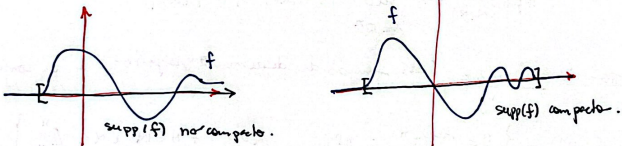
\includegraphics[height=0.8\textheight, width=0.8\textwidth, keepaspectratio]{./Images/support_types_04.png}
	\end{center}
	\caption{representações de funções com suporte compacto e não compacto.}
\end{figure}

\begin{example}
	Se K for um compacto de \(\mathbb{R}^{n}\) com interior não vazio, indiquemos por \(\mathcal{C}_{c}^{\infty}(K)\) o conjunto das funções \(f\in \mathcal{C}^{\infty}(\mathbb{R}^{n})\) com suporte \(\mathrm{supp}(f)\subseteq K\) (consequentemente, suporte compacto), tais que f sejam todas identicamente nulas em \(\mathbb{R}^{n}\setminus{K}.\)
	\begin{figure}[H]
		\begin{center}
			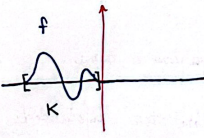
\includegraphics[height=0.5\textheight, width=0.5\textwidth, keepaspectratio]{./Images/compact_support_04.png}
		\end{center}
		\caption{exemplo de f no conjunto \(\mathcal{C}_{c}^{\infty}(K)\) definido.}
	\end{figure}

	Como consequência, quando munido da topologia de \(\mathcal{C}^{\infty}(\mathbb{R}^{n})\), o espaço \(\mathcal{C}_{c}^{\infty}(K)\) é um subespaço fechado, portanto também é completo. Para isso, note que, se \(f_{n}\equiv 0\) em \(\mathbb{R}^{n}\setminus{K}\) e \(\{f_{n}\}_{n}\) converge para f pontualmente, então f é identicamente nula em \(\mathbb{R}^{n}\setminus{K},\) garantindo que \(\mathrm{supp}(f)\subseteq K.\)
\end{example}

\end{document}
